\title{Лекция 5\\Представление в базе знаний множеств и операций над ними}   
\author[]{Шункевич Д.В.}
\institute[]{Белорусский государственный университет информатики и радиоэлектроники}

\begin{frame}
	\titlepage
\end{frame}

\begin{frame}{\\Содержание лекции}
	
	\topline
	\justifying
	Типология множеств, рефлексивное множество. Ориентированное множество, декартово произведение множеств. Атрибуты, кортежи и классические кортежи. Мощность, бесконечные и конечные множества (без представления в базе знаний). Отношения над множествами, равенство. Операции над канторовскими множествами. Операции над мультимножествами. Булеан множества, его мощность. Представление в базе знаний.
\end{frame}

\begin{frame}{\\Понятие множества}
	\topline
	\justifying
	Под \textbf{\textit{множеством}} понимается соединение в некое целое M определённых хорошо различимых предметов m нашего созерцания или нашего мышления (которые будут называться ``элементами'' множества M).\\
	\bigskip
	\textbf{\textit{множество}} -- мысленная сущность, которая связывает одну или несколько сущностей в целое.\\
	\bigskip
	Более формально \textbf{\textit{множество}} -- это абстрактный математический объект, состоящий из элементов. Связь множеств с их элементами задается бинарным ориентированным отношением \textbf{\textit{принадлежность*}}.\\
	\bigskip
	В Теории множеств \textbf{\textit{множество}} считается неопределяемым понятием, его можно только пояснить.
	\vspace{-3em}
\end{frame}

\begin{frame}{\\Задание множеств}%задание множеств 1 
	\topline
	\justifying
	
	
	\textbf{\textit{множество}} может быть полностью задано следующими тремя способами:
	
	\begin{textitemize}
	\item путем перечисления (явного указания) всех его элементов (очевидно, что таким способом можно задать только конечное множество)
    \end{textitemize}

\vspace{2em}   

	\scnrelfrom{изображение}{
		
			\begin{center}
				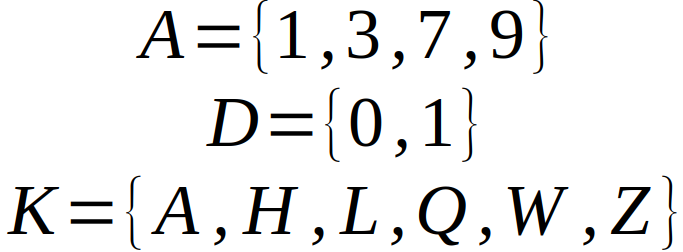
\includegraphics[width=40mm]{figures/sd_sets/enumeration_of_set.png}
			
	\end{center}
  
}    
\vspace{-4em}   	 
\end{frame}

\begin{frame}%задание множест2
	
	\begin{textitemize}	    
	\item с помощью определяющего высказывания, содержащего описание общего характеристического свойства, которым обладают все те и только те объекты, которые являются элементами (т.е. принадлежат) задаваемого множества.
    \end{textitemize}

\vspace{2em}

	\scnrelfrom{изображение}{
		
		\begin{center}
			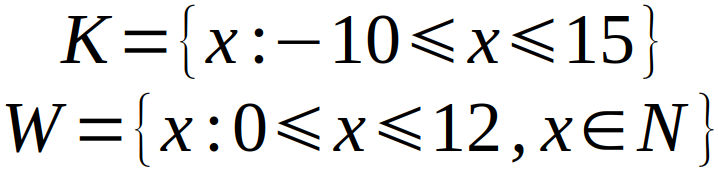
\includegraphics[width=45mm]{figures/sd_sets/descriptionProperties_set.png}
		\end{center}
	}
\vspace{-6em}      
\end{frame}

\begin{frame}%задание множест3
	
	\begin{textitemize}
	\item с помощью теоретико-множественных операций, позволяющих однозначно задавать новые множества на основе уже заданных (это операции объединения, пересечения, разности множеств и др.)
	\end{textitemize}

\vspace{2em}

    \scnrelfrom{изображение}{
     	
     	\begin{center}
     		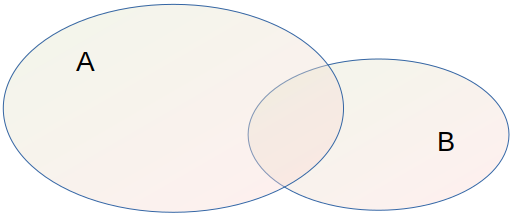
\includegraphics[width=40mm]{figures/sd_sets/unitiSets.png}
     	\end{center}
     }

\vspace{0.2em}
 
    \scnrelfrom{изображение}{
    	
    	\begin{center}
    		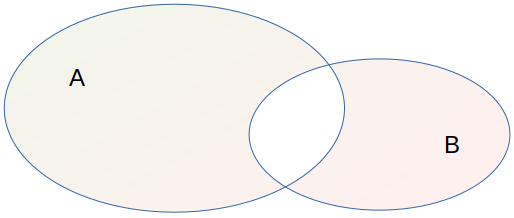
\includegraphics[width=40mm]{figures/sd_sets/intersectionSets.png}
    	\end{center}
    }

 
    
	\vspace{-4em}
\end{frame}

\begin{frame}{\\Принадлежность}
	\topline
	\justifying
	\begin{SCn}
		\scnheader{принадлежность*}
		\scnidtf{принадлежность элемента множеству*}
		\scniselement{бинарное отношение}
		\scniselement{ориентированное отношение}
	\end{SCn}
	
	\textbf{\textit{принадлежность*}} – это бинарное ориентированное отношение, каждая связка которого связывает множество с одним из его элементов.\\
	\bigskip
	Элементами отношения \textbf{\textit{принадлежность*}} в \textit{SC-коде} по умолчанию являются \textbf{\textit{базовые sc-дуги}} (позитивные постоянные константные sc-дуги принадлежности).
\end{frame}

\begin{frame}{\\Классификация множеств}
	\topline
	\justifying
	\begin{SCn}
	\scnheader{множество}
	\begin{scnrelfromset}{разбиение}
		\scnitem{конечное множество}
		\scnitem{бесконечное множество}
	\end{scnrelfromset}
	\begin{scnrelfromset}{разбиение}
		\scnitem{множество без кратных элементов}
		\scnitem{мультимножество}
	\end{scnrelfromset}
	\begin{scnrelfromset}{разбиение}
		\scnitem{кортеж}
		\scnitem{неориентированное множество}
	\end{scnrelfromset}
	\end{SCn}
\end{frame}

\begin{frame}{\\Конечность множеств}
	\topline
	\justifying
	\begin{SCn}
	\scnheader{конечное множество}
	\scnidtf{множество с конечным числом элементов}
	\end{SCn}

	\textbf{\textit{конечное множество}} – это \textit{множество}, количество элементов которого конечно, т.е. существует неотрицательное целое число \textit{k}, равное количеству элементов этого множества.
	\vspace{-\baselineskip}
	\begin{SCn}	
	\scnheader{бесконечное множество}
	\scnidtf{множество с бесконечным числом элементов}
	\begin{scnrelfromset}{разбиение}
		\scnitem{счетное множество}
		\scnitem{несчетное множество}
	\end{scnrelfromset}
	\end{SCn}
	\textbf{\textit{бесконечное множество}} – это \textit{множество}, в котором для любого натурального числа \textit{n} найдётся конечное подмножество из \textit{n} элементов.

\end{frame}

\begin{frame}{\\Счетность множеств}
	\topline
	\justifying
	\textbf{\textit{счетное множество}} -- это \textit{бесконечное множество}, для которого существует \textit{взаимно однозначное соответствие} с натуральным рядом чисел.

	\begin{SCn}	
	\scnheader{несчетное множество}
	\scnidtf{континуальное множество}
	\end{SCn}

	\textbf{\textit{несчетное множество}} -- это \textit{бесконечное множество}, элементы которого невозможно пронумеровать натуральными числами.
\end{frame}

\begin{frame}{\\Кратность множеств}%множество без кратных элементов
	\topline
	\justifying
\begin{SCn}
	\scnheader{множество без кратных элементов}
	\scnidtf{классическое множество}
	\scnidtf{множество, состоящее из разных элементов}
\end{SCn}
	\scntext{пояснение}{\textbf{\textit{множество без кратных элементов}} -- это \textit{множество}, для каждого элемента которого существует только одна пара принадлежности, выходящая из знака этого множества в указанный элемент.}
\vspace{5.5em}
\end{frame}

\begin{frame}%мультимножество
	
	\begin{SCn}	
		\scnheader{мультимножество}
		\scnidtf{множество, имеющее кратные вхождения хотя бы одного элемента}
		\scnidtf{множество, по крайней мере один элемент которого входит в его состав многократно}
	\end{SCn}
	
	\scntext{пояснение}{\textbf{\textit{мультимножество}} -- это \textit{множество}, для которого существует хотя бы одна кратная пара принадлежности, выходящая из знака этого множества.}
\end{frame}
	
\begin{frame}%кратность принадлежности		
	\begin{SCn}
\scnheader{кратность принадлежности}
\scnidtf{кратность принадлежности элемента}
\scnidtf{кратность вхождения элемента во множество}
\scniselement{параметр}
    \end{SCn}

\scntext{пояснение}{\textbf{\textit{кратность принадлежности}} -- \textit{параметр}, значением которого являются числовые величины, показывающие сколько раз входит тот или иной элемент в рассматриваемое множество. Элементами данного параметра являются классы \textit{позитивных sc-дуг принадлежности}, связывающих данное множество с элементом, кратность вхождения которого в данное множество мы хотим задать. %TODO Пример

Таким образом, кратное вхождение элемента в мультимножество может быть задано как явным указанием \textit{позитивных sc-дуг принадлежности} этого элемента данному \textit{множеству}, так и «склеиванием» этих дуг в одну и включением ее в некоторый класс \textbf{\textit{кратности принадлежности}}.}
\vspace{6em}
\end{frame}

\begin{frame}%кратность принадлежности пример
\scnrelfrom{описание примера}{
	\begin{center}
	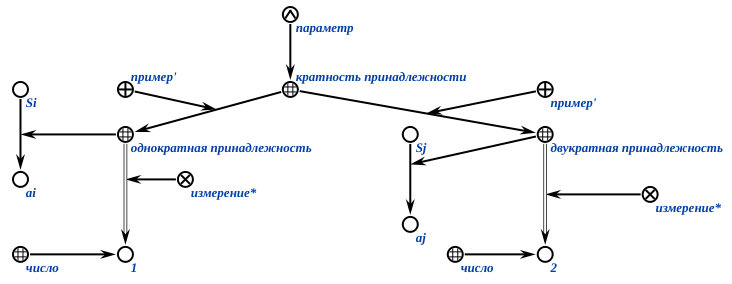
\includegraphics[width=120mm]{figures/sd_sets/multiplicityOfMembership.png}
	\end{center}
}
\vspace{-1em}
\end{frame}

\begin{frame}{\\Нечеткое и четкое множество }%нечеткое и четкое множество
\topline
\justifying
	\begin{SCn}		
\scnheader{нечеткое множество}
\end{SCn}

\scntext{пояснение}{\textbf{\textit{нечеткое множество}} – это \textit{множество}, которое представляет собой совокупность элементов произвольной природы, относительно которых нельзя точно утверждать – обладают ли эти элементы некоторым характеристическим свойством, которое используется для задания этого нечеткого множества. Принадлежность элементов такому множеству указывается при помощи \textit{нечетких позитивных sc-дуг принадлежности}.}

\vspace{-1em}
\begin{SCn}
	\scnheader{четкое множество}
\end{SCn}
\scntext{пояснение}{\textbf{\textit{четкое множество}} – это \textit{множество}, принадлежность элементов которому достоверна и указывается при помощи \textit{четких позитивных sc-дуг принадлежности}.}
\vspace{-2em}
\end{frame}

\begin{frame}{\\Семейство множеств}%семейсво множеств 
	\topline
	\justifying
	\begin{SCn}
		\scnheader{семейство множеств}
		\scnidtf{множество множеств}
		\scnsuperset{класс классов}
	\end{SCn}
	
	\scntext{пояснение}{\textbf{\textit{семейство множеств}} – это \textit{множество}, элементами которого являются знаки множеств.}
\vspace{8em}
\end{frame}

\begin{frame}{\\Свойства отношений на множестве}%свойства отношений на множестве 
	\topline
	\justifying
	
\begin{SCn}
\scnheader{нерефлексивное множество}
\end{SCn}

\scntext{пояснение}{\textbf{\textit{нерефлексивное множеств}} – это \textit{множество}, знак которого не является элементом этого множества}



\begin{SCn}
\scnheader{рефлексивное множество}
\end{SCn}

\scntext{пояснение}{\textbf{\textit{рефлексивное множеств}} – это \textit{множество}, знак которого является элементом этого множества}
\vspace{-1em}

\end{frame}

\begin{frame}{\\Множество}%множество 
	\topline
	\justifying
	
   \begin{SCn}	
   \scnheader{множество}
   \scnsuperset{пустое множество}
   \scnsuperset{синглетон}
   \scnsuperset{пара}
   \scnsuperset{тройка}
   \end{SCn}

\vspace{8.5em}
\end{frame}	

\begin{frame}{\\Пустое множество} %пустое множество
  \topline
  \justifying
  
   \begin{SCn}
   	\scnheader{пустое множество}
   	\scniselement{мощность множества}
   \end{SCn}

    \scntext{пояснение}{\textbf{\textit{пустое множество}} – это \textit{множество}, которому не принадлежит ни один элемент.}
    
\vspace{8.5em}
\end{frame}
    	
\begin{frame}{\\Синглетон}%синглетон 
	\topline
	\justifying
	
	\begin{SCn}
	\scnheader{синглетон}
	\scniselement{мощность множества}
	\scnidtf{множество мощности 1}
	\scnidtf{одноэлементное множество}
	\scnidtf{одномощное множество}
    \scnidtf{множество, мощность которого равна 1}
    \scnidtf{множество, имеющее мощность равную единице}
    \scnidtf{синглетон из sc-элемента} 
    \scnidtf{sc-синглеон}
    \scnsubset{конечное множество}
    \end{SCn}


   \scntext{пояснение}{\textbf{\textit{синглетон}} – это \textit{множество}, состоящее из одного элемента.}
    	
    	
\end{frame}

\begin{frame}{\\Пара}%пара
	\topline
\justifying
    \begin{SCn}
	\scnheader{пара}
	\scniselement{мощность множества}
	\scnidtf{множество мощности два}
	\scnidtf{двухэлементное множество}
	\scnidtf{двумощное множество}
	\scnsubset{конечное множество}
    \end{SCn}

    \scntext{пояснение}{\textbf{\textit{пара}} – это \textit{множество}, состоящее из двух элементов.}
\vspace{4.5em} 	
    	
\end{frame}

\begin{frame}{\\Тройка} %тройка	
	\topline
\justifying
	
	\begin{SCn}
	\scnheader{тройка}
	\scniselement{мощность множества}
	\scnidtf{тройка}
	\scnidtf{множество мощности три}
	\scnsubset{конечное множество}
	\end{SCn}

	\scntext{пояснение}{\textbf{\textit{тройка}} – это \textit{множество}, состоящее из трех элементов.}
\vspace{6em}
\end{frame}

\begin{frame}{\\Мощность}%мощность множества //невместилось 
		\topline
	\justifying
	
	\begin{SCn}
    \scnheader{мощность множества}
    \scnidtf{кардинальное число}
    \scnidtf{общее число вхождений элементов в заданное множество}
    \scnidtf{класс эквивалентности, элементами которого являются знаки всех тех и только тех множеств, которые имеют одинаковую мощность}
    \scnidtf{класс эквивалентности, соответствующий отношению быть парой множеств, имеющих одинаковую мощность (равномощность множеств)}
    \scnidtf{величина мощности множеств}
    \scnidtf{трансфинитное число}
    \scnidtf{мощность по Кантору}
    \scniselement{параметр}
    \end{SCn}
\end{frame}

\begin{frame}
	\scnheader{мощность множества}
    \scntext{пояснение}{\textbf{\textit{мощность множества}} – это \textit{параметр}, элементами которых являются \textit{множества}, имеющие одинаковое количество элементов. Значением данного параметра является числовая величина, задающая количество элементов, входящих в данный класс множеств, т.е. по сути, количество \textit{позитивных sc-дуг принадлежности}, выходящих из данного \textit{множества}.}
\vspace{-2em}	
\end{frame}
	
\begin{frame}{\\Кортеж}%кортеж
	\topline
\justifying	
	
	\begin{SCn}
    \scnheader{кортеж}
    \scnidtf{вектор}
    \end{SCn}


    \scntext{пояснение}{\textbf{\textit{кортеж}} – это множество, представляющее собой упорядоченный набор элементов, т.е. такое множество, порядок элементов в котором имеет значение. Пары принадлежности элементов \textbf{\textit{кортежу}} могут дополнительно принадлежать каким-либо \textit{ролевым отношениям}, при этом, в рамках каждого \textbf{\textit{кортежа}} должен существовать хотя бы один элемент, роль которого дополнительно уточнена \textit{ролевым отношением}.}
\vspace{2em}
\end{frame}






%%Отношения на множествах
\begin{frame}{\\Отношения на множествах}%включение
\topline
\justifying	
	\begin{SCn}
    \scnheader{включение*}
    \scnidtf{быть подмножеством*}
    \scniselement{бинарное отношение}
    \scniselement{ориентированное отношение}
    \scniselement{транзитивное отношение}
    \scnrelfrom{область определения}{множество}
    \scnsuperset{строгое включение*}
    \end{SCn}

    \scntext{определение}{\textbf{\textit{включение*}} – это бинарное ориентированное отношение, каждая связка которого связывает два множества. Будем говорить, что \textit{Множество Si} \textbf{\textit{включает*}} в себя \textit{Множество Sj} в том и только том случае, если каждый элемент \textit{Множества Sj} является также и элементом \textit{Множества Si}.}
    \vspace{-3em}
\end{frame} 

\begin{frame}%рисунок включения
    \scnrelfrom{описание примера}{
    \begin{center}
    	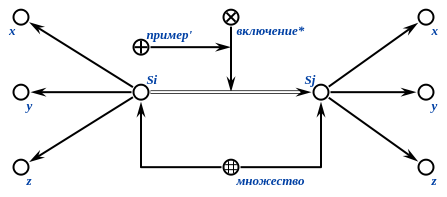
\includegraphics[width=100mm]{figures/sd_sets/inclusion.png}
    \end{center}}
    

    \begin{scnindent}
    \scntext{пояснение}{Множество {Sj} включается во множество \textit{Si}.}
    \end{scnindent}
\vspace{-1em}
\end{frame}

\begin{frame}%строгое включение
	
	\begin{SCn}
	\scnheader{строгое включение*}
	\scnidtf{строгое включение множеств*}
	\scnsubset{включение*}
	\scniselement{бинарное отношение}
	\scniselement{ориентированное отношение}
	\scnrelfrom{область определения}{множество}
	\end{SCn}

    \scntext{определение}{\textbf{\textit{строгое включение*}} – это \textit{бинарное ориентированное отношение}, областью определения которого является семейство всевозможных множеств. Будем говорить, что \textit{Множество Si} \textbf{\textit{строго включает*}} в себя \textit{Множество Sj} в том и только том случае, если каждый элемент \textit{Множество Sj} является также и элементом \textit{Множество Si}, при этом существует хотя бы один элемент \textit{Множество Si}, не являющийся элементом \textit{Множество Sj}.}
    \vspace{3em}
\end{frame}

\begin{frame}%рисунок строгое включение
	
    \scnrelfrom{описание примера}{
	\begin{center}
	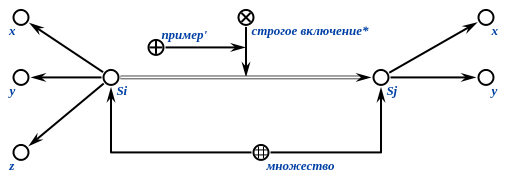
\includegraphics[width=22em]{figures/sd_sets/strictInclusion.png}
    \end{center}}
    
    \begin{scnindent}
    \scntext{пояснение}{Множество \textit{Sj} строго включается во множество \textit{Si}.}
    \end{scnindent}

\scnrelfrom{изображение}{
	\begin{center}
		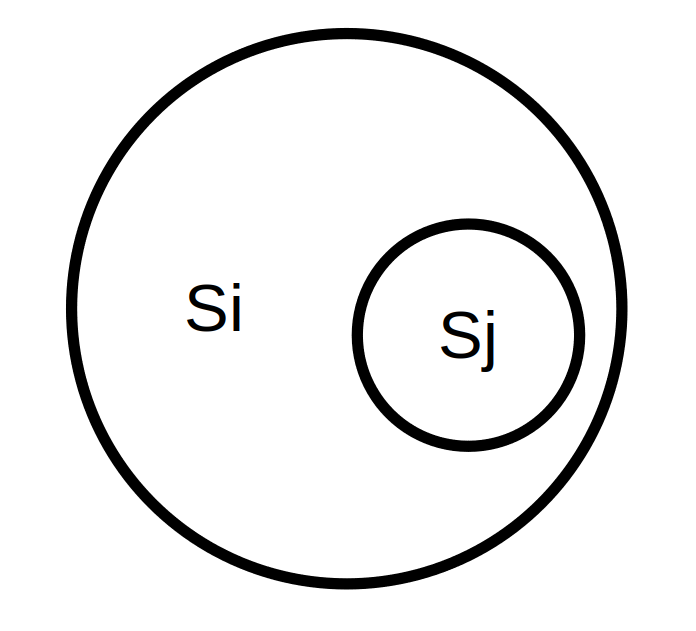
\includegraphics[width=7em]{figures/sd_sets/inclusion2.png}
\end{center}}

\vspace{-1.5em}
\end{frame}

\begin{frame}%равенство множеств
	
	\begin{SCn}
		\scnheader{равенство множеств*}
		\scniselement{бинарное отношение}
		\scniselement{неориентированное отношение}
		\scnidtf{быть равными множествами*}
    \end{SCn}

    \scntext{определение}{\textbf{\textit{равенство множеств}}* -- бинарное неориентированное отношение, выражающее отношение равенства множеств.
	
	Любые два множества являются равными множествами тогда и только тогда, когда первое является включением второго и второе является включением первого.}
\vspace{9em}
\end{frame}

\begin{frame}%рисунок равенства множеств
    \scnrelfrom{описание примера}{
    \begin{center}
%не влазит
	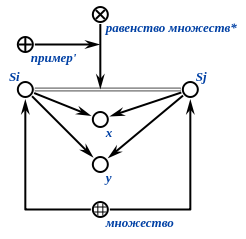
\includegraphics[width=50mm]{figures/sd_sets/equalityOfSets.png}
    \end{center}}

    \begin{scnindent}
    \scntext{пояснение}{Множество \textit{Si} равно множеству \textit{Sj}.}
    \end{scnindent}

\end{frame}

\begin{frame}%булеан
	
	\begin{SCn}
		\scnheader{булеан*}
		\scnidtf{булеан множества*}
		\scnidtf{семейство всевозможных подмножеств заданного множества*}
		\scniselement{бинарное отношение}
		\scniselement{ориентированное отношение}
	\end{SCn}

    \scntext{определение}{\textbf{\textit{булеан*}} – это \textit{бинарное ориентированное отношение} между множеством и некоторым семейством множеств, каждое из которых является подмножеством первого множества.}
    
    \scnrelfrom{описание примера}{
    \begin{center}
    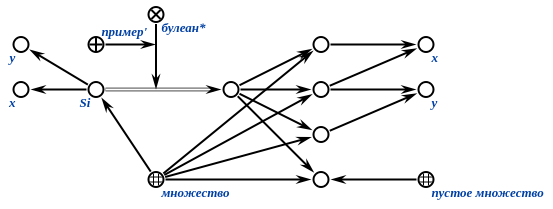
\includegraphics[width=100mm]{figures/sd_sets/boulean.png}
    \end{center}}

\end{frame}

\begin{frame}%семейство подмножеств
   
   \begin{SCn}
	\scnheader{семейство подмножеств*}
	\scnidtf{семейство подмножеств заданного множества*}
	\scniselement{бинарное отношение}
	\scniselement{ориентированное отношение}
	\scnsuperset{булеан*}
    \end{SCn}

    \scntext{определение}{\textbf{\textit{семейство подмножеств*}} – это \textit{бинарное ориентированное отношение} между множеством и некоторым семейством множеств, каждое из которых является подмножеством первого множества.}
   
	
    \scnrelfrom{описание примера}{
    \begin{center}
    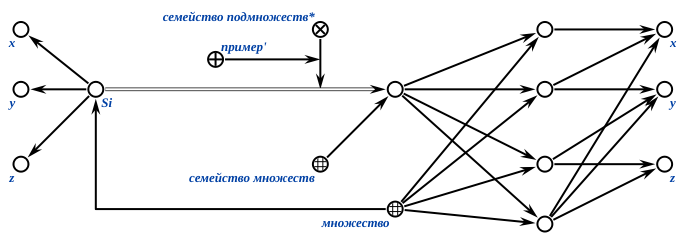
\includegraphics[width=100mm]{figures/sd_sets/familyOfSubsets.png}
    \end{center}}

\end{frame}





%%Операции на множествах
\begin{frame}{\\Операции на множествах}%объединение
\topline
\justifying	
	\begin{SCn}
		\scnheader{объединение*}
		\scnidtf{объединение множеств*}
		\scniselement{квазибинарное отношение}
		\scniselement{ориентированное отношение}
	\end{SCn}

    \scntext{определение}{\textbf{\textit{объединение*}} – это \textit{квазибинарное ориентированное отношение}, областью определения которого является семейство всевозможных множеств. Будем говорить, что \textit{Множество Si} является объединением \textit{Множество Sj} и \textit{Множество Sk} тогда и только тогда, когда любой элемент \textit{Множество Si} является элементом или \textit{Множество Sj} или \textit{Множество Sk}.}
    \vspace{1em}
   
\end{frame}

\begin{frame}%рисунок объединение	
 
  \scnrelfrom{описание примера}{
 	\begin{center}
 		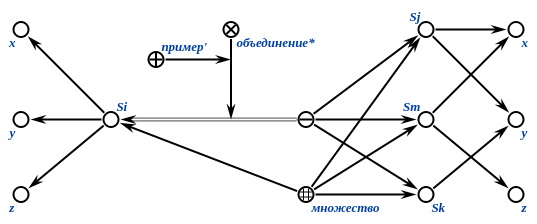
\includegraphics[width=75mm]{figures/sd_sets/union.png}
 \end{center}}
    \begin{scnindent}
    	\scntext{пояснение}{Множество \textit{Si} является объединением множеств \textit{Sj}, \textit{Sk} и \textit{Sm}.}
    \end{scnindent}

    \scnrelfrom{изображение}{
    \begin{center}
    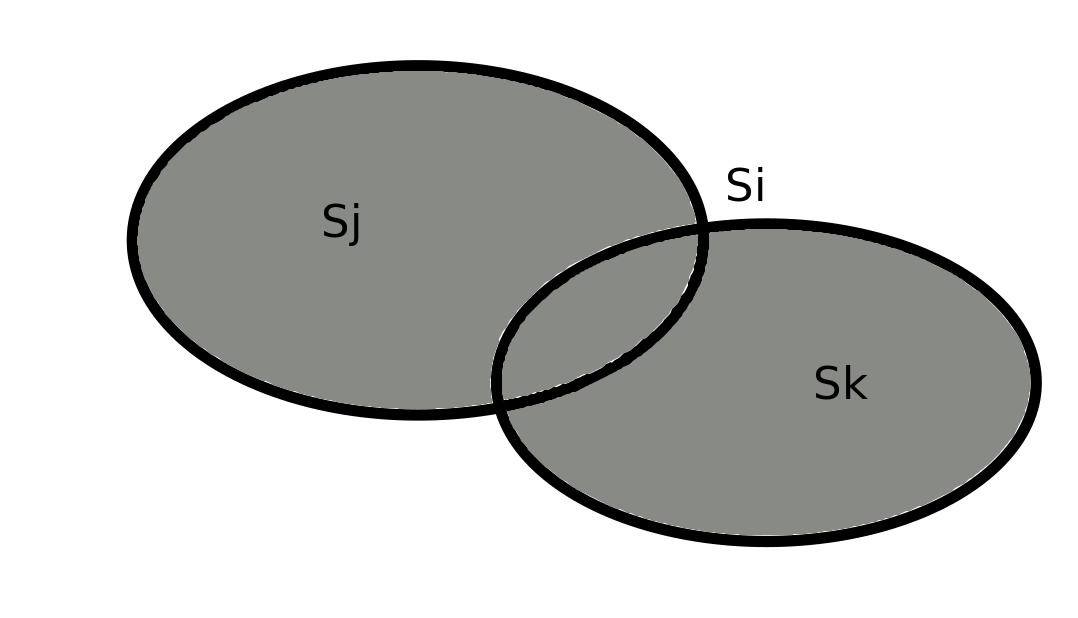
\includegraphics[width=45mm]{figures/sd_sets/union2.png}
    \end{center}}
\vspace{-3em}
\end{frame}

%%еще не сделано ошибка
\begin{frame}%разбиение 
	\begin{SCn}
\scnheader{разбиение*}
\scnidtf{разбиение  множества*}
\scnidtf{объединение попарно непересекающихся множеств*}
\scnidtf{декомпозиция множества*}
\scniselement{квазибинарное отношение}
\scniselement{ориентированное отношение}
\scniselement{отношение декомпозиции}
\end{SCn}
\end{frame}

\begin{frame}
	\scnheader{разбиение*}
\scntext{определение}{\textbf{\textit{разбиение*}} – это \textit{квазибинарное ориентированное отношение}, областью определения которого является семейство всевозможных множеств. В результате разбиения множества получается множество попарно непересекающихся множеств, объединение которых есть исходное множество.\\
	Семейство множеств \{\textit{S1…, Sn}\} является разбиением множества \textit{Si} в том и только том случае, если:

%\begin{SCn}
%	\begin{scnitemize}
		\item семейство \{\textit{S1…, Sn}\} является семейством \textit{попарно непересекающихся множеств};
		\item семейство \{\textit{S1…, Sn}\} является покрытием множества \textit{Si} (или другими словами, множество \textit{Si} является \textit{объединением} множеств, входящих в указанное выше семейство)
%	\end{scnitemize}
%\end{SCn}
}
\end{frame}

\begin{frame}%разбиение2 + рисунок
	    
    \scnrelfrom{описание примера}{
    \begin{center}
    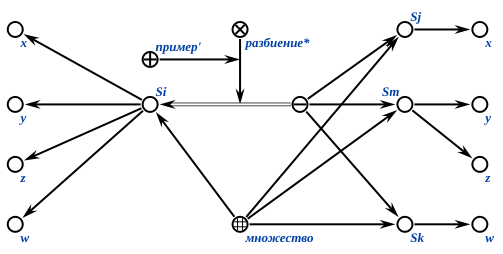
\includegraphics[width=40mm]{figures/sd_sets/split.png}
    \end{center}}

    \begin{scnindent}
    \scntext{пояснение}{Множество \textit{Si} разбивается на множества \textit{Sj}, \textit{Sk} и \textit{Sm}.}
    \end{scnindent}

    \scnrelfrom{изображение}{
    \begin{center}
	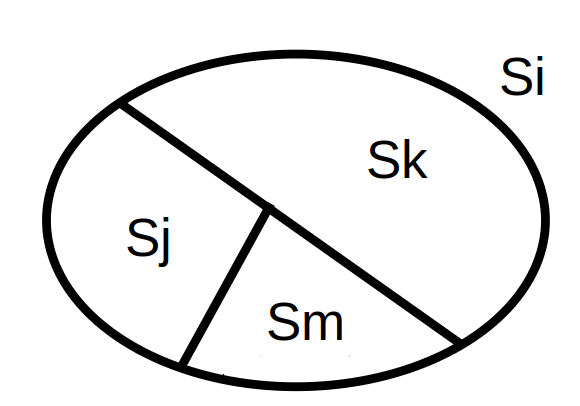
\includegraphics[width=40mm]{figures/sd_sets/split2.png}
    \end{center}}

\end{frame}

\begin{frame}%пересечение
	
	\begin{SCn}
	\scnheader{пересечение*}
	\scnidtf{пересечение множеств*}
	\scniselement{квазибинарное отношение}
	\scniselement{ориентированное отношение}
	\end{SCn}
    
    \scntext{определение}{\textbf{\textit{пересечение*}} – это операция над множествами, аргументами которой являются два или большее число множеств, а результатом является множество, элементами которого являются все те и только те сущности, которые одновременно принадлежат каждому множеству, которое входит в семейство аргументов этой операции.\\
	Будем говорить, что \textit{Множество Si} является пересечением \textit{Множество Sj} и \textit{Множество Sk} тогда и только тогда, когда любой элемент \textit{Множество Si} является элементом \textit{Множество Sj} и элементом \textit{Множество Sk}.}
\vspace{6em}
\end{frame}

\begin{frame}%пересечение рисунки
	
    \scnrelfrom{описание примера}{
    \begin{center}
	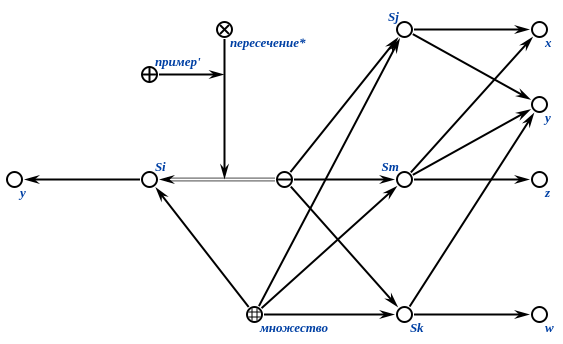
\includegraphics[width=70mm]{figures/sd_sets/intersection.png}
    \end{center}}

    \begin{scnindent}
    \scntext{пояснение}{Множество \textit{Si} является результатом пересечения множеств \textit{Sj}, \textit{Sk} и \textit{Sm}.}
    \end{scnindent}

    \scnrelfrom{изображение}{
    \begin{center}
	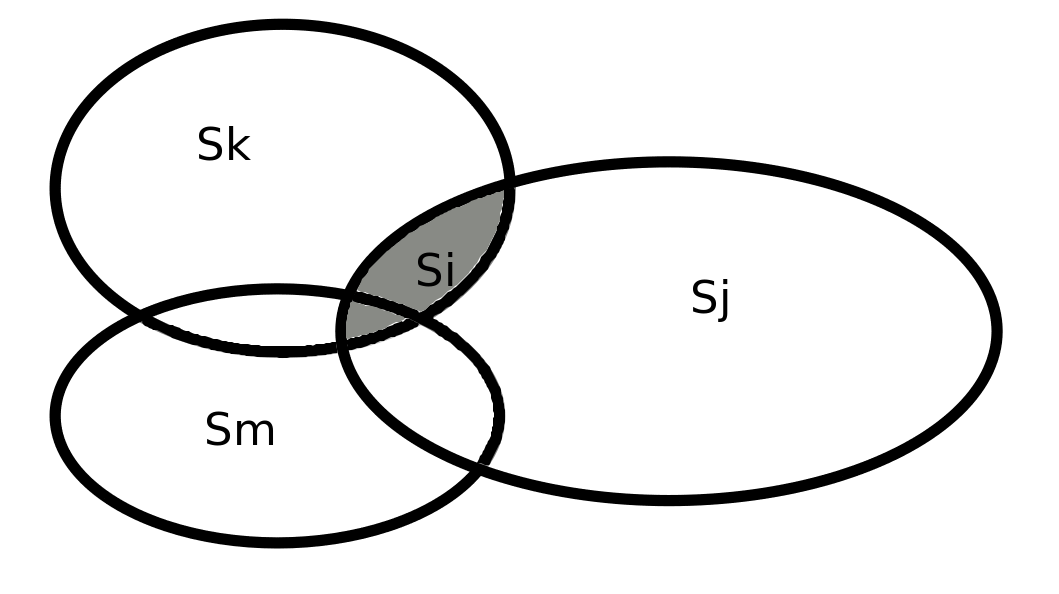
\includegraphics[width=40mm]{figures/sd_sets/intersection2.png}
    \end{center}} 

\end{frame}

\begin{frame}%разность
	
	\begin{SCn}
	\scnheader{разность множеств*}
	\scniselement{бинарное отношение}
	\scniselement{ориентированное отношение}
	\end{SCn}

   \scntext{определение}{\textbf{\textit{разность множеств*}} – это \textit{бинарное ориентированное отношение}, связывающее между собой \textit{ориентированную пару}, первым элементом которой является уменьшаемое множество, вторым -- вычитаемое множество, и множество, являющееся результатом вычитания вычитаемого из уменьшаемого, в которое входят все элементы первого множества, не входящие во второе множество.}
  \vspace{10em} 
\end{frame}   

\begin{frame}%разность рисунок 

   \scnrelfrom{описание примера}{
   \begin{center}
   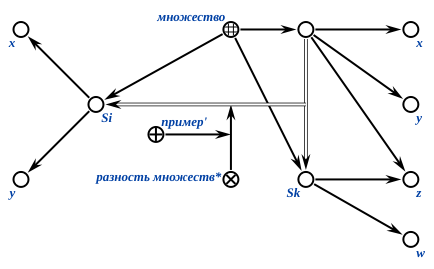
\includegraphics[width=75mm]{figures/sd_sets/setDifference.png}
   \end{center}}

   \begin{scnindent}
   \scntext{пояснение}{Множество \textit{Si} является результатом разности множеств \textit{Sj} и \textit{Sk}.}
   \end{scnindent}

   \scnrelfrom{изображение}{
   \begin{center}
   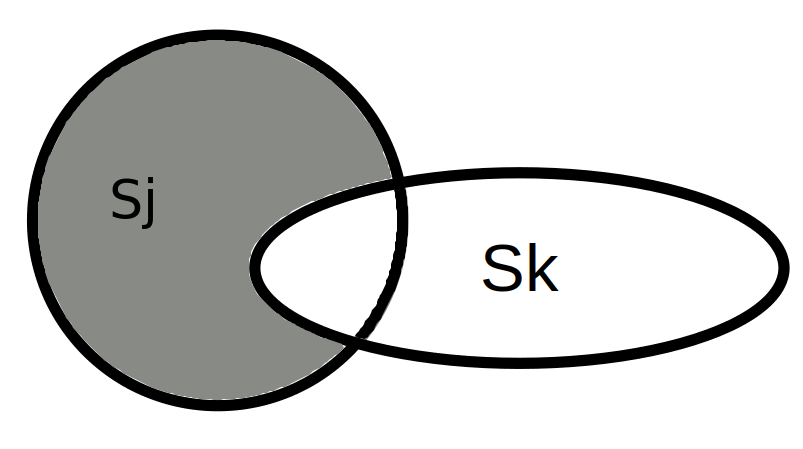
\includegraphics[width=40mm]{figures/sd_sets/setDifference2.png}
   \end{center}}

\end{frame}

\begin{frame}%сим.разность
	
	\begin{SCn}
	\scnheader{симметрическая разность множеств*}
	\scniselement{бинарное отношение}
	\scniselement{ориентированное отношение}
	\end{SCn}

    \scntext{определение}{\textbf{\textit{симметрическая разность множеств*}} – это \textit{бинарное ориентированное отношение}, связывающее между собой \textit{пару} множеств и множество, являющееся результатом симметрической разности элементов указанной пары. Будем называть \textit{Множество Si} результатом симметрической разности \textit{Множества Sj} и \textit{Множества Sk} тогда и только тогда, когда любой элемент \textit{Множества Si} является или элементом \textit{Множества Sj} или \textit{Множества Sk}, но не является элементом обоих множеств.}
\vspace{8em}
\end{frame}

\begin{frame}%сим.разность рис
	
    \scnrelfrom{описание примера}{
    \begin{center}
	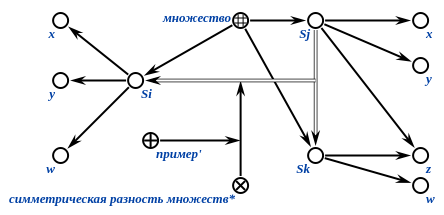
\includegraphics[width=75mm]{figures/sd_sets/symmetricDifferenceOfSets.png}
	\end{center}}

	\scntext{пояснение}{Множество \textit{Si} является результатом симметрической разности множеств \textit{Sj} и \textit{Sk}.}
	
    \scnrelfrom{изображение}{
    \begin{center}
	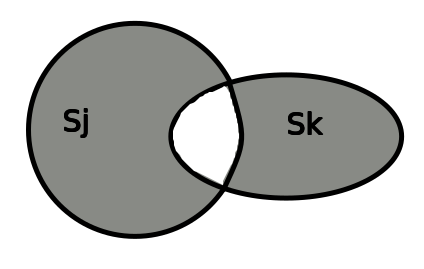
\includegraphics[width=35mm]{figures/sd_sets/symmetricDifferenceOfSets2.png}
    \end{center}}

\end{frame}

\begin{frame}%декартово произведение
	
	\begin{SCn}
	\scnheader{декартово произведение*}
	\scnidtf{декартово произведение множеств*}
	\scnidtf{прямое произведение множеств*}
	\scniselement{бинарное отношение}
	\scniselement{ориентированное отношение}
	\end{SCn}

    \scntext{определение}{\textbf{\textit{декартово произведение*}} – это \textit{бинарное ориентированное отношение} между \textit{ориентированной парой} множеств и \textit{множеством}, элементами которого являются всевозможные упорядоченные пары, первыми элементами которых являются элементы первого из указанных множеств, вторыми – элементы второго из указанных множеств.}
\vspace{10em}
\end{frame}

\begin{frame}%декартово произведение рис
	
    \scnrelfrom{описание примера}{
    \begin{center}
	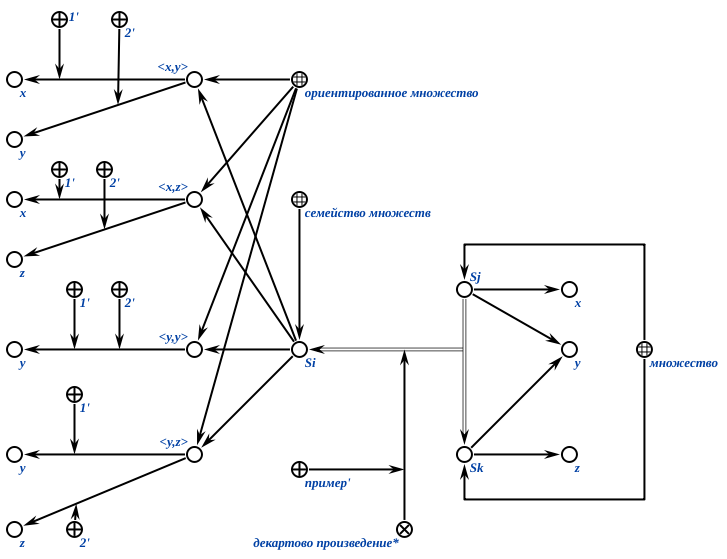
\includegraphics[width=80mm]{figures/sd_sets/cartesianMultiplication.png}
    \end{center}}

    \begin{scnindent}
    \scntext{пояснение}{Множество \textit{Si} является результатом декартова произведения множеств \textit{Sj} и \textit{Sk}.}
    \end{scnindent}

\end{frame}






%Пересекающиеся множества
\begin{frame}{\\Пересекающиеся множества}%пара пересек.множ.
\topline
\justifying	
	\begin{SCn}
	\scnheader{пара пересекающихся множеств*}
    \scniselement{бинарное отношение}
    \scniselement{неориентированное отношение}
    \end{SCn}

   \scntext{пояснение}{\textbf{\textit{пара пересекающихся множеств*}} – \textit{бинарное неориентированное отношение} между двумя \textit{множествами}, имеющими непустое \textit{пересечение*}.} 
   
   \scntext{определение}{\textbf{\textit{пара пересекающихся множеств*}} – \textit{бинарное неориентированное отношение} между двумя \textit{множествами}, имеющими, по крайней мере, один общий для этих двух множеств элемент.}
\vspace{1em}
\end{frame}
 
\begin{frame}%пара пересек.множ.рис.

   \scnrelfrom{описание примера}{
   \begin{center}
   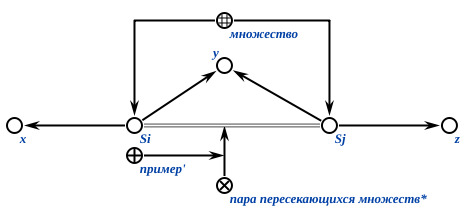
\includegraphics[width=80mm]{figures/sd_sets/pairOfIntersectingSets.png}
   \end{center}}


   \begin{scnindent}
   \scntext{пояснение}{Множество \textit{Si} и множество \textit{Sj} являются парой пересекающихся множеств.}
   \end{scnindent}
   
   \scnrelfrom{изображение}{
   \begin{center}	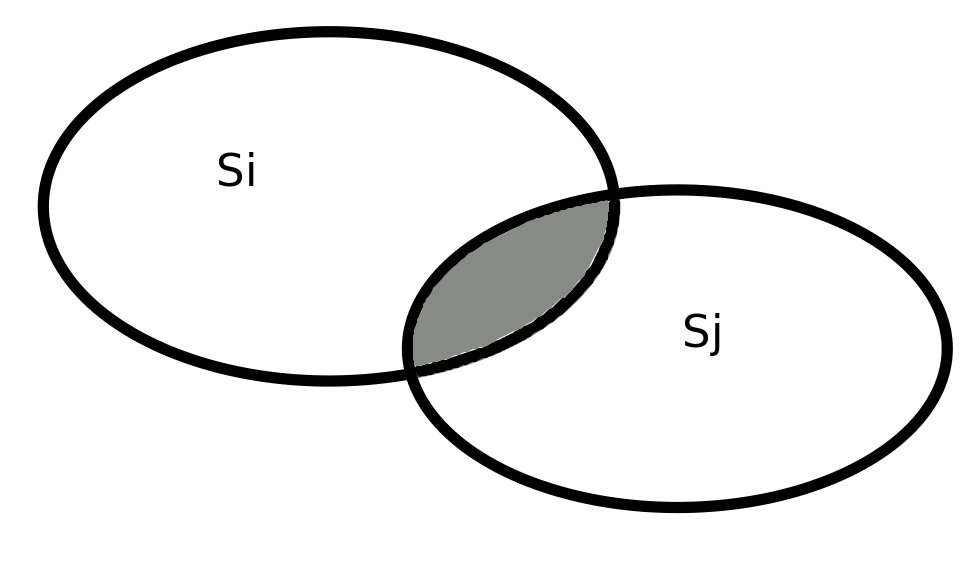
\includegraphics[width=40mm]{figures/sd_sets/pairOfIntersectingSets2.png}
   \end{center}}
\vspace{-2em}
\end{frame}

\begin{frame}%попарно пересек.множ.
	
	\begin{SCn}
	\scnheader{попарно пересекающиеся множества*}
	\scnidtf{семейство попарно пересекающихся множеств*}
	\scnsuperset{пересекающиеся множества*}
	\scniselement{отношение}
	\end{SCn}

    \scntext{определение}{\textbf{\textit{попарно пересекающиеся множества*}} – семейство множеств, каждая пара которых является парой пересекающихся множеств, т.е. каждая пара которых имеет хотя бы один общий элемент}
    
    \scntext{примечание}{Не каждое \textit{семейство попарно пересекающихся множеств*} является \textit{семейством пересекающихся множеств*}, хотя обратное верно.}
   
  
\vspace{9em}
\end{frame}

\begin{frame}%попарно пресек.множ.рис.%не влезло
	    
      \scnrelfrom{изображение}{
    	\begin{center}
    		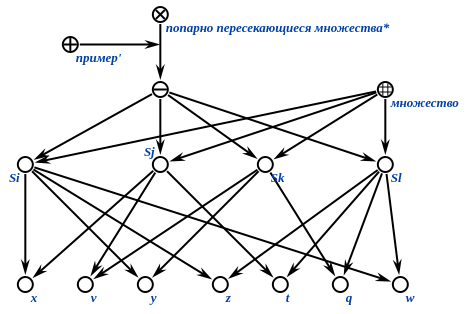
\includegraphics[width=50mm]{figures/sd_sets/pairwiseIntersectingSets.png}
  \end{center}}

   \begin{scnindent}
   \scntext{пояснение}{Множества \textit{Si}, \textit{Sj}, \textit{Sk} и \textit{Sl} являются попарно пересекающимися множествами.}
   \end{scnindent}


   \scnrelfrom{изображение}{
   \begin{center}
   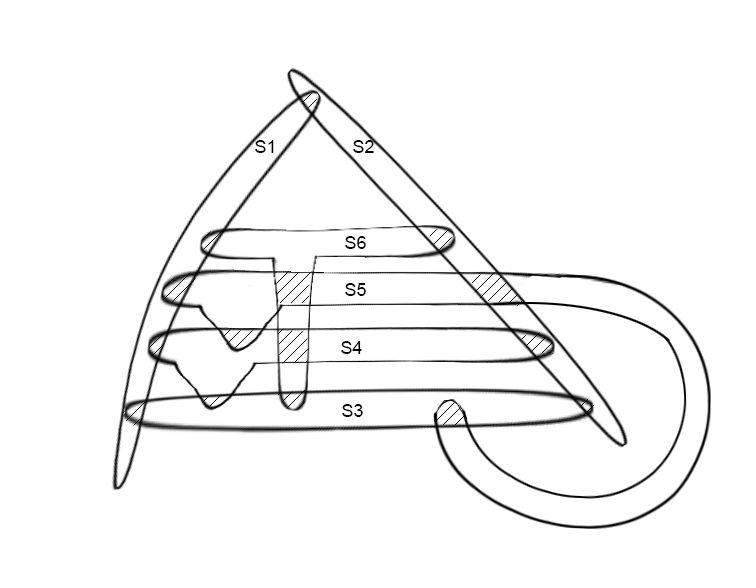
\includegraphics[width=40mm]{figures/sd_sets/pairwiseIntersectingSets2.png}
   \end{center}}

\end{frame}

\begin{frame}%пересекающиеся множества
	
	\begin{SCn}
    \scnheader{пересекающиеся множества*}
    \scnidtf{семейство пересекающихся множеств*}
    \scnidtf{быть семейством пересекающихся множеств*}
    \scnidtf{семейство множеств, имеющих по крайней мере один элемент, являющийся общим для всех этих множеств*}
    \scnsuperset{попарно пересекающиеся множества*}
    \end{SCn}

    \scntext{определение}{\textbf{\textit{пересекающиеся множества*}} – это семейство множеств, имеющих по крайней мере один общий для всех этих множеств элемент}

   
\vspace{14em}
\end{frame}

\begin{frame}%пересекающиеся множества рис.

   \scnrelfrom{описание примера}{
  	\begin{center}
  		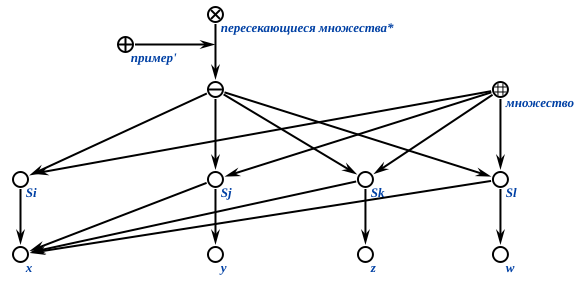
\includegraphics[width=100mm]{figures/sd_sets/intersectingSets.png}
  \end{center}}
  \begin{scnindent}
  	\scntext{пояснение}{Множества \textit{Si}, \textit{Sj}, \textit{Sk} и \textit{Sl} являются пересекающимися множествами.}
  \end{scnindent}
\vspace{2em}
\end{frame}

\begin{frame}%пара непересек.множ.
	
	\begin{SCn}
    \scnheader{пара непересекающихся множеств*}
    \scniselement{бинарное отношение}
    \scniselement{неориентированное отношение}
    \end{SCn}

    \scntext{определение}{\textbf{\textit{пара непересекающихся множеств*}} – это \textit{бинарное неориентированное отношение} между \textit{множествами}, результатом \textit{пересечения*} которых есть пустое множество.}
    
  
\vspace{15em}
\end{frame}

\begin{frame}%пара непересек.множ.рис.
	
       \scnrelfrom{описание примера}{
   	\begin{center}
   		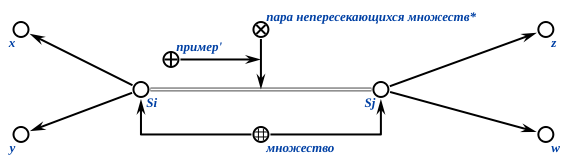
\includegraphics[width=90mm]{figures/sd_sets/pairOfNonIntersectingSets.png}
   \end{center}}
   
   
   \begin{scnindent}
   	\scntext{пояснение}{Множества \textit{Si} и \textit{Sj} являются парой непересекающихся множеств.}
   \end{scnindent}
   
   \scnrelfrom{изображение}{
   	\begin{center}
   		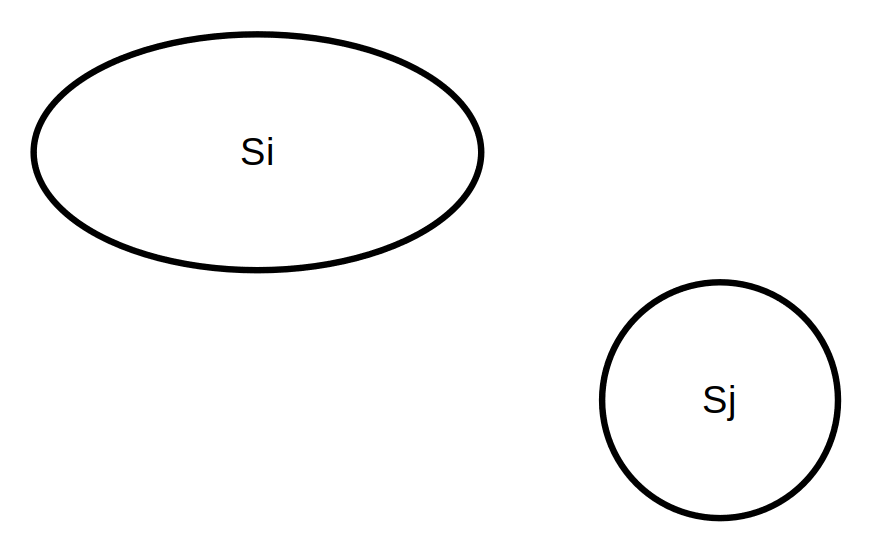
\includegraphics[width=40mm]{figures/sd_sets/pairOfNonIntersectingSets2.png}
   \end{center}} 

    

\end{frame}

\begin{frame}%попарно непересек.множ.
	
	\begin{SCn}
	\scnheader{попарно непересекающиеся множества*}
    \scnidtf{семейство попарно непересекающихся множеств*}
    \scnsubset{непересекающиеся множества*}
    \end{SCn}

    \scntext{определение}{\textbf{\textit{попарно непересекающиеся множества*}} – семейство множеств, каждая пара которых является парой непересекающихся множеств, т.е. каждая пара которых не имеет ни одного общего элемента}
    \vspace{15em}
\end{frame}

\begin{frame}%попарно непересек.множ.рис.    
    \scnrelfrom{изображение}{
    \begin{center}	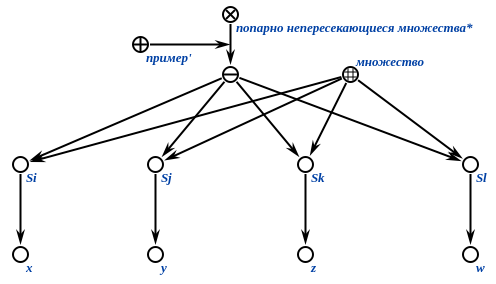
\includegraphics[width=90mm]{figures/sd_sets/pairwiseNonIntersectingSets.png}
    \end{center}}

    \begin{scnindent}
    \scntext{пояснение}{Множества \textit{Si}, \textit{Sj}, \textit{Sk} и \textit{Sl} являются попарно непересекающимися множествами.}
    \end{scnindent}

\end{frame}

\begin{frame}%непересек.множ.
	
	\begin{SCn}
    \scnheader{непересекающиеся множества*}
    \scnidtf{семейство непересекающихся множеств*}
    \scnidtf{быть семейством непересекающихся множеств*}
    \end{SCn}

    \scntext{определение}{\textbf{\textit{непересекающиеся множества*}} – это семейство множеств, не имеющих ни одного общего элемента для всех этих множеств}
    \vspace{15em}
\end{frame}

\begin{frame}    
    \scnrelfrom{изображение}{
    \begin{center}
  	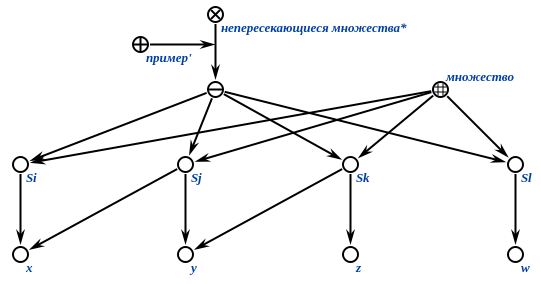
\includegraphics[width=90mm]{figures/sd_sets/nonIntersectingSets.png}
    \end{center}}

 	\scntext{пояснение}{Множества \textit{Si}, \textit{Sj}, \textit{Sk} и \textit{Sl} являются непересекающимися множествами.}

\end{frame}
